\documentclass[10pt,journal,compsoc]{IEEEtran}

\usepackage{CJKutf8}

\usepackage{tabularx}

\usepackage{enumitem}

\usepackage[nocompress]{cite}

\usepackage{listings}

\usepackage{color}

\lstset{
    basicstyle=\ttfamily,
    literate={├}{|}1 {─}{--}1 {│}{|}1 {└}{+}1
}

\ifCLASSINFOpdf
  \usepackage[pdftex]{graphicx}
\else
  \usepackage[dvips]{graphicx}
\fi

\usepackage{amsmath}

\usepackage[caption=false,font=footnotesize,labelfont=sf,textfont=sf]{subfig}

\newcommand\MYhyperrefoptions{
bookmarks=true,
bookmarksnumbered=true,
pdfpagemode={UseOutlines},
plainpages=false,
pdfpagelabels=true,
colorlinks=true,
linkcolor={black},
citecolor={black},
urlcolor={black},
pdftitle={Speech Synthesis Based on GAN},
pdfsubject={Typesetting},
pdfauthor={Zhang Wentao, Guo Yachen},
pdfkeywords={TTS, GAN, Speech, Synthesis}
}

\hyphenation{op-tical net-works semi-conduc-tor}

\begin{document}

\title{Speech Synthesis Based on GAN}

\author{
Zhang Wentao,
Guo Yachen
}

\markboth{Speech Synthesis Based on GAN, SoarCraft, June 2021} {}

\IEEEtitleabstractindextext{
\begin{abstract}

The rapid development of neural networks has brought more possibilities for applying artificial intelligence. In recent years, Generative Adversarial Networks (GANs) have attracted global attention due to their unsupervised training mechanism and the potential for development through mutual adversarial enhancement. Speech generation models have wide practical significance and can be applied to the underlying implementation of functions such as text-to-speech or virtual voices. Currently, most mature speech models in mainstream deep learning models are based on Convolutional Neural Networks (CNNs). The main research on GAN models is currently focused on image training, while related work on audio training is still in its early stages. This paper explores the feasibility of speech generation using GANs and designs a speech generation model based on GANs to obtain high-quality generated speech, laying the foundation for subsequent other speech functions.

This paper first elaborates on the development of GANs. It provides a brief introduction to basic GAN and speech synthesis concepts. Next, it describes the design of a GAN model composed of a generator based on the Google speech synthesis model and a discriminator based on spectral normalization. It provides a detailed explanation and analysis of the related debugging results. Finally, this paper evaluates the generated results and analyzes the related engineering problems.

\hfill June 5, 2021
\end{abstract}

\begin{IEEEkeywords}
TTS, GAN, Speech, Synthesis
\end{IEEEkeywords}}

\maketitle

\IEEEdisplaynontitleabstractindextext

\IEEEpeerreviewmaketitle

\IEEEraisesectionheading{\section{Introduction}\label{sec:introduction}}

\subsection{Research Background and Significance.}

\IEEEPARstart{I}{n} recent years, the rapid development of neural networks has brought more possibilities for the practical application of artificial intelligence \cite{1}. Among them, the Generative Adversarial Network (GAN) proposed by Ian Goodfellow in 2014 has attracted widespread attention in the industry. Its unsupervised and label-free characteristics make it simpler, more efficient, and more potent than other neural network models. Since 2014, numerous GAN-based optimization models have emerged. The Deep Convolutional GAN (DCGAN) has achieved excellent training results, leading GANs into the mainstream development stage. Currently, GANs have shown great success in various fields \cite{2}.

Speech generation technology has a relatively early starting point, with the appearance of a new computer speech output system in the late 1970s. This system used the most basic speech units to concatenate relevant synthetic speech. Subsequently, various models based on speech feature synthesis have continuously emerged. The most representative one is the DECTalk, successfully developed in 1982.

In recent years, GANs have made significant progress in image generation. However, GANs have received little attention in the audio field. Currently, most mature speech models are based on Convolutional Neural Networks (CNNs), with prominent examples being Google's WaveNet \cite{3} model and Baidu's Deep Voice model. However, these models have drawbacks, such as not supporting parallel training and slow speed.

Due to the limited exploration of GANs in speech synthesis, this paper focuses on exploring the feasibility of using GANs for speech generation and designing a speech generation model based on GANs. The aim is to simplify the training difficulty and improve the speed and reliability of training through the unique adversarial and balancing properties of GAN models. This is done to obtain good-quality generated speech and lay a foundation for subsequent speech-related functionalities.

\subsection{Review of Current Research}

Currently, research on GANs in China mainly focuses on applications and reviews. However, the overall number of papers is still relatively small. According to the search results on the China National Knowledge Infrastructure (CNKI), there are only 2685 records of GAN-related papers published on the platform. Most research efforts focus on how to optimize GAN-derived models and implement them in practical applications, with only a few papers independently designing GAN-derived models, such as the master's thesis by Zixuan Wang in 2020 titled "FLOWGAN: Research on Key Technologies for Encrypted Traffic Recognition Based on Generative Adversarial Network." Research on GANs in the field of speech in China is scarce. Only 56 records of GAN-related papers on speech were published on CNKI, all of which are application-oriented, with no independent model design.

Research on GANs abroad mainly focuses on applications, reviews, and model design. GANs have spawned various models with different characteristics, such as the Deep Convolutional GAN (DCGAN) based on deep convolutional neural networks and the Conditional GAN (cGAN) with relevant conditional constraints. Research on GANs in audio synthesis has made some progress abroad, with two high-quality representative models being WaveGAN and GANSynth. Both successfully applied GANs to simple audio datasets. The former used a GAN model to generate raw audio, obtaining a dataset of spoken digit commands from zero to nine. The latter created a dataset of single-note recordings from various instruments by training a GAN to generate the reversible spectrogram of musical notes. Neekhara et al. proposed an adversarial vocoder model that can synthesize amplitude spectrograms from melody spectrograms generated by Tacotron 2, incorporating related local weighting and phase estimation techniques. Overall, although GANs have made some development in speech synthesis, research on GANs in the field of speech synthesis still needs to be a popular topic \cite{4}.

\subsection{Research Content and Research Methods}

There is still significant room for the development of GAN in speech synthesis. This paper focuses on designing a GAN model consisting of a generator based on the Google speech synthesis model and a discriminator based on spectral normalization. For any neural network training in deep learning frameworks, feature extraction issues must be taken seriously. Learning analysis can only be conducted when the dataset has effective identifying features. This paper designs a speech preprocessing format that matches the GAN model from the perspective of the Mel-Frequency domain to assist the GAN model in better training. Experimental contents were then conducted, and the related debugging results were analyzed and explained in detail. Finally, the results were analyzed, and complex engineering issues were discussed accordingly.

This paper conducted a wide-ranging investigation of the development of GAN in speech synthesis and the use of related models through the survey method to understand the research status and related issues. Secondly, this paper analyzed the experimental research of other researchers on GAN through the literature research method and reasonably borrowed other, more complete GAN models to assist in designing the core of this paper's GAN and other related modules. Meanwhile, relevant technical reference documents were studied and referred to for help with the required technical content for the experiment. Finally, this paper used experimental and comparative methods for the related model design. It evaluated the rationality of the model through a series of experiments, analyzing the related experimental data to evaluate the model's validity and selecting the best model design based on data comparison.

\section{Introduction to Related Technical}

\subsection{Generative Adversarial Networks}

\subsubsection{Overview of GAN in Speech}

GAN, proposed by Ian Goodfellow in 2014, is a novel implicit neural network training model inspired by the Nash equilibrium in game theory \cite{5}. GAN consists of two independent neural networks \cite{6}, the generator, and the discriminator.

\begin{figure}
    \centering
    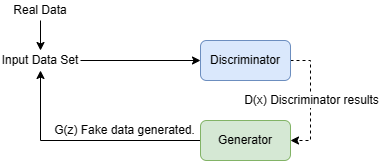
\includegraphics[scale=0.6] {PNG/2-1.png}
    \caption{GAN schematic}
    \label{fig:2-1}
\end{figure}

The discriminator plays a role similar to traditional deep learning models, which is to distinguish and verify data in the dataset while learning the main features of the data to improve its ability to distinguish data. The generator's task is to generate fake data, attempting to fool the discriminator's discernment. The generator's data comes entirely from random noise distributed uniformly, which is expanded through a reverse neural network model to generate data similar to the target data. When the discriminator judges the data, it gives a probability indicating the degree of truthfulness, limited between 0 and 1. After the discriminator judges the fake data generated by the generator, the probability value is fed back to the generator. The generator adjusts the relevant parameters according to the probability value for better generation results \cite{7}. The objective function of GAN is:

\begin{equation}
    \begin{aligned}
        &min_G max_D V(D, G) = \\
        &E_{x-P(x)} [\log {D(x)}] + E_{z-P(z)} [\log {\Bigl(1-D \bigl(G(z)\bigr) \Bigr)}]
    \end{aligned}
\end{equation}

\begin{figure}
    \centering
    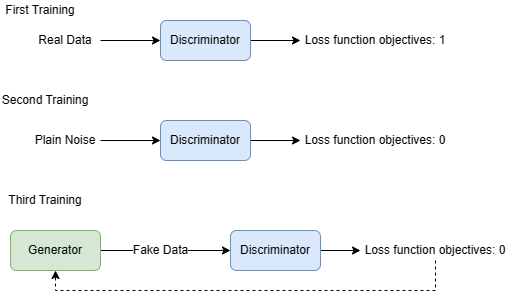
\includegraphics[scale=0.5] {PNG/2-2.png}
    \caption{GAN three times training decomposition diagram}
    \label{fig:2-2}
\end{figure}

GANs avoid using complex Markov chains for gradient acquisition, instead employing backpropagation algorithms to compute gradients based on the probability values of the degree of truth or falsity mentioned above and to adjust the relevant parameters. The structure of GAN is simple, and the learning cost is low without excessive complex inference calculations. However, it can generate objectively effective data results due to its adversarial characteristics. The data results generated by GAN also have high quality, and compared with other deep learning models, GAN has greater development advantages.

While GANs have many advantages, they also inevitably have some drawbacks. First, the training of GANs must effectively control the learning speed of the generator and discriminator to be balanced. When the learning speed of the generator is faster than that of the discriminator, the generator can easily fool the discriminator, making it difficult to adjust and optimize subsequently; when the learning speed of the discriminator is faster than that of the generator, the discriminator generally gives lower scores, causing the generator to lose its optimization direction and unable to optimize effectively and rationally, resulting in blind optimization or even reverse optimization. Second, GANs suffer from mode collapse, i.e., some samples with only minor differences are treated as multiple samples with significant differences, leading to convergence to a single result; and GANs also have the problem of gradient disappearance, i.e., when there is no overlap or negligible overlap between real and generated samples, the divergence of the objective function optimized by the network becomes a constant \cite{8}.

Compared with other traditional speech synthesis areas and other traditional deep learning network frameworks, GANs can more effectively conduct unsupervised training, allowing computers to find core internal relationships independently without the need for excessive data preprocessing. At the same time, traditional speech synthesis models tend to use phoneme elements for synthesis and concatenation, which rely heavily on basic preprocessing and analysis of each sample, while GANs are relatively robust, able to resist certain disadvantages of improper sample processing, and have higher training speed than traditional speech synthesis systems.

\subsubsection{Activation Functions}

The precursor of activation functions was used to simulate digital circuit switches. Due to its similarity to the behavior of linear perceptrons in neural networks, it was applied to map the output of a neuron to the next one using a special function relationship. The core purpose of activation functions is to introduce nonlinearity to neural network models, enabling them to approximate any nonlinear function. Currently, there are several popular activation functions, including:

\begin{enumerate}
    \item Sigmoid function

\begin{equation}
    \begin{aligned}
        sigmoid: f(x) = \frac{1}
                             {1 + e^x}
    \end{aligned}
\end{equation}

The sigmoid function has the advantage of simple derivative calculation and a stable output mapping range between (0, 1), resulting in a limited output range and stable optimization. However, it suffers from severe function saturation and gradient vanishing problems, which means that the gradient value approximates zero when the function approaches a huge value, making it difficult to optimize the model effectively.

\begin{figure}
    \centering
    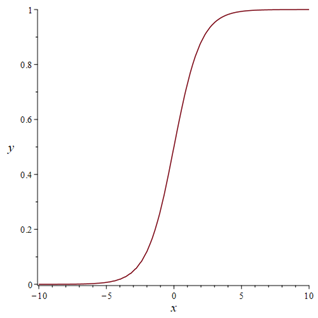
\includegraphics[scale=0.6] {PNG/2-3.png}
    \caption{Sigmoid function}
    \label{fig:2-3}
\end{figure}

    \item Hyperbolic tangent function

\begin{equation}
    \begin{aligned}
        tanh: f(x) = \frac{e^x - e^{-x}}
                         {e^x + e^{-x}}
    \end{aligned}
\end{equation}

The hyperbolic tangent function (tanh) is an optimization of the sigmoid function, which addresses the non-zero mean in the sigmoid. However, it still needs to solve the problem of gradient vanishing in the sigmoid function \cite{9}.

\begin{figure}
    \centering
    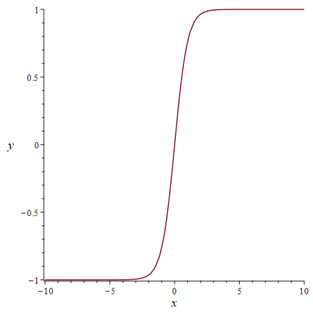
\includegraphics[scale=0.6] {PNG/2-4.png}
    \caption{tanh function}
    \label{fig:2-4}
\end{figure}

    \item Rectified Linear Unit

\begin{equation}
    \begin{aligned}
        ReLU = max(0, x)
    \end{aligned}
\end{equation}

The Rectified Linear Unit (ReLU) function \cite{10} is currently one of the most popular activation functions used in neural networks. It effectively addresses the problem of vanishing gradients present in earlier activation functions. Its simplified function design also results in significantly faster computation. Moreover, compared to the sigmoid and tanh functions, ReLU exhibits much faster convergence due to its inherent one-sided saturation property \cite{11}.

However, ReLU also has some disadvantages. First, its output does not satisfy zero-mean normalization. Second, it is prone to the Dead ReLU Problem, where certain neurons' respective parameters may never be activated or updated during the later stages of training.

\begin{figure}
    \centering
    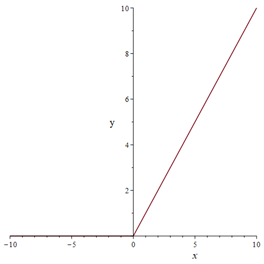
\includegraphics[scale=0.6] {PNG/2-5.png}
    \caption{ReLU function}
    \label{fig:2-5}
\end{figure}

    \item Leaky ReLU

\begin{equation}
    \begin{aligned}
        Leaky ReLU = max(ax, x)
    \end{aligned}
\end{equation}

The Leaky Rectified Linear Unit (Leaky ReLU) function, an optimized version of the ReLU function, was proposed for acoustic modeling. It addresses the Dead ReLU Problem by introducing a small slope to the negative direction. While theoretically, Leaky ReLU has all the advantages of ReLU. It has yet to be proven that Leaky ReLU is always superior to ReLU in practical applications \cite{12}.

\begin{figure}
    \centering
    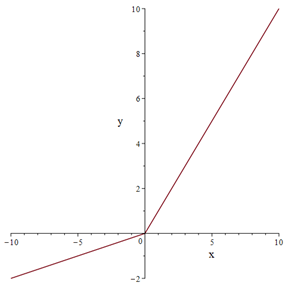
\includegraphics[scale=0.6] {PNG/2-6.png}
    \caption{Leaky ReLU function $(\alpha = 0.2)$}
    \label{fig:2-6}
\end{figure}

    \item Parameterized ReLU

Parameterized Rectified Linear Unit (PReLU) is an activation function that designs the slope parameter alpha in Leaky ReLU as a learnable parameter. This provides more flexibility but may require more adjustment costs overall.

    \item Exponential Linear Unit

\begin{equation}
    \begin{aligned}
        ELU: f(x) = 
        \begin{cases}
            x & \text{if } x > 0 \\
            \alpha (e^x - 1) & \text{else}
        \end{cases}
    \end{aligned}
\end{equation}

The Exponential Linear Unit (ELU) theoretically combines all the advantages of the activation above functions, achieving the goal of output zero-mean normalization and having one-sided saturation for effective convergence. However, its more complex equation increases the computational burden. Its practical application depends on testing and selection based on the specific situation.

\begin{figure}
    \centering
    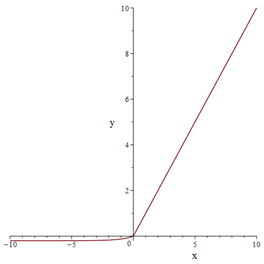
\includegraphics[scale=0.6] {PNG/2-7.png}
    \caption{ELU function $(\alpha = 0.2)$}
    \label{fig:2-7}
\end{figure}

\end{enumerate}

\subsubsection{Optimizer}

The optimizer is used to adjust the parameters in a model. It calculates the values of parameters that need to be adjusted. It adjusts the relevant parameters in the neural network to achieve the optimal solution for the model.

\begin{enumerate}
    \item Gradient Descent

\begin{equation}
    \begin{aligned}
        W_{t + 1} = W_t + \eta_t \Delta J (W_t)
    \end{aligned}
\end{equation}

In formula:

\begin{itemize}[label={}]
    \item $W_t$ --- Learning parameters at time t
    \item $\eta_t$ --- Learning Rate
    \item $\Delta J (W_t)$ --- Gradient
\end{itemize}

The Standard Gradient Descent algorithm (GD) is the most primitive and fundamental method for adjusting parameters by continually reducing them along the gradient direction, minimizing cost parameters. However, the GD method has many drawbacks, including slow training speed due to updating parameters at every step and the risk of getting stuck in a local optimum, finding saddle points or local minima rather than the global minimum.

    \item Batch Gradient Descent

\begin{equation}
    \begin{aligned}
        W_{t + 1} = W_t + \eta_t \sum_{i=1}^{n} {\Delta J (W_t, X^{(i)}, Y^{(i)})}
    \end{aligned}
\end{equation}

In formula:

\begin{itemize}[label={}]
    \item $X^{(i)}$ --- Input Sample
    \item $Y^{(i)}$ --- Output Sample
\end{itemize}

Batch Gradient Descent (BGD) combines parameter updates with all input samples, adjusting only after batch sample inputs. This speeds up the overall training process and allows for basic regional adjustments, reducing the likelihood of getting stuck in local optima.

    \item Stochastic Gradient Descent

\begin{align}
    W_{t + 1} = W_t - \eta_t g_t \\
    g_t = \Delta J_{i_s} (W_t, X^{(i_s)}, Y^{(i_s)}) \ \ \ i_s\in \{ 1, 2, \ldots, n \}
\end{align}

In formula:

\begin{itemize}[label={}]
    \item $i_s$ --- Randomly Selected Direction
\end{itemize}

Stochastic Gradient Descent (SGD) is a method that utilizes randomness and perturbations to converge on the optimal solution ultimately. It can address the local optima that are susceptible to being disturbed by stochastic perturbations. However, more is needed to solve the problem of local optima fundamentally. Additionally, due to its stochastic nature, the computational speed of SGD is significantly improved. However, randomness also introduces noise, which can cause the direction of weight updates to be incorrect.

    \item Mini-Batch Gradient Descent

Mini-Batch Gradient Descent (MBGD) is a combined approach that integrates the benefits of both Batch Gradient Descent (BGD) and Stochastic Gradient Descent (SGD). Compared to BGD, MBGD reduces the size of the batch by utilizing a subset of the samples, accelerating the overall training speed.

    \item Momentum

\begin{align}
    {m_t = \mu \times m}_{t - 1} + g_t \\
    \Delta \theta_t = -\eta \times m_t
\end{align}

The momentum method simulates momentum in physics by introducing a new variable to accumulate the previous momentum instead of the corresponding gradient. This technique effectively optimizes the issue of GD-type algorithms not accumulating data from previous iterations, thereby accelerating the overall convergence. Additionally, momentum can enhance the update magnitude and help escape from local minima, effectively alleviating situations where local optima exist.

    \item Nesterov

\begin{align}
    g_t = \nabla_{\theta_{t-1}} f(\theta_{t-1} - \eta \times \mu \times m_{t-1})
\end{align}

Nesterov's method is an improvement upon the momentum method. It allows for considering the previous variable $m_{t-1}$ in calculating the gradient, which introduces a certain correction amount.

    \item Adaptive Gradient

\begin{align}
    n_t = n_{t-1} + g_t^2 \\
    \Delta \theta_t = - \frac{\eta}
                             {\sqrt{n_t + \epsilon}} \times g_t
\end{align}

In formula:

\begin{itemize}[label={}]
    \item $\epsilon$ --- Global Learning Rate
\end{itemize}

Adaptive Gradient (AdaGrad) is the first algorithm to introduce adaptive adjustments. It includes a constraint term that can appropriately amplify when gradients are small in the early stages and appropriately reduce when gradients are too large in the later stages. AdaGrad is suitable for sparse gradients; however, it still relies on the set learning rate.

    \item Adadelta

This algorithm is an improvement upon AdaGrad. Compared to AdaGrad, Adadelta only accumulates fixed-size terms rather than all gradient squares. Moreover, Adadelta no longer requires a learning rate by employing a similar operation to the Newton iteration method. Its advantages include effectively accelerating early-stage training, but it can cause severe shaking near the optimal solution in the later stages.

    \item RMSprop

\begin{align}
    AdaGrad: r \gets r+g \bigodot g \\
    RMSprop: r \gets \rho r + (1 - \rho)g \bigodot g
\end{align}

In formula:

\begin{itemize}[label={}]
    \item $\rho$ --- Decay factor, used to control how much historical gradient information is obtained
\end{itemize}

It is also a modified version of the AdaGrad algorithm. Experimentally, RMSprop's algorithm has proven more effective than AdaGrad in speed and accuracy.

    \item Adam \cite{13}

This algorithm is a combination of the momentum method and the adaptive learning rate method. It possesses both the accelerating convergence feature of the momentum method and the automatic learning rate adjustment feature. It is one of the most widely used optimization algorithms due to its stronger optimization efficiency and wider applicability.

\end{enumerate}

\subsubsection{Loss function}

The loss function is used to evaluate the difference between the predicted values of a model and the true values. It is an important function for measuring the performance of a model. 

\begin{enumerate}
    \item 0 - 1 function

\begin{align}
    L \bigl (Y, f(x) \bigr) = 
    \begin{cases}
        1 \text{, } Y \neq f(x) \\
        0 \text{, } Y = f(x)
    \end{cases}
\end{align}

When the predicted value equals the true value, the result is 0, and 1 otherwise. This function is often used to determine the number of corresponding errors directly. However, since achieving perfect results in practical situations is impossible, some requirements are often relaxed in daily use, allowing for a certain degree of difference.

\begin{align}
    L \bigl (Y, f(x) \bigr) = 
    \begin{cases}
        1 \text{, } |Y - f(x)| \geq T \\
        0 \text{, } |Y - f(x)| < T
    \end{cases}
\end{align}

    \item Absolute value loss function

\begin{align}
    L \bigl (Y, f(x) \bigr) = |Y - f(x)|
\end{align}

The absolute loss function is calculated as the difference between the predicted and true values. This type of loss function can describe the loss situation in contrast to the 0-1 loss function. However, it still has drawbacks, such as a need for more control over the numerical range in the case of large differences and potential difficulty in identifying significant features.

    \item Logarithmic loss function

\begin{align}
    L \bigl (Y, f(x) \bigr) = - \log {P (Y | f(x))}
\end{align}

The logarithmic function, also known as the logistic regression function, is a mapping function that maps the value range of the absolute loss function to the probability distribution range and thus can represent the probability distribution very well. However, it has some drawbacks, such as low robustness.

    \item MSELoss

\begin{align}
    L \bigl (Y, f(x) \bigr) = \bigl( Y - f(x) \bigr)^2
\end{align}

The mean squared error function (MSE loss) computes the squared difference between the predicted and true values. 

    \item L1 Loss \cite{14}

\begin{align}
    L(Y, f(x)) = \frac{\sum_{i=1}^{n} {|y_i + y_i^p|}}
                      {n}
\end{align}

The mean absolute error loss function (L1 loss) is used to compute the average loss value for a set of results. This type of function is commonly used when there are multiple output values.

\end{enumerate}

\subsubsection{Convolution}

Convolution techniques are developed to deal with the analysis of localized features. It focuses on analyzing the features of each local part and extract. It simplifies them to obtain a summary of localized information. This technique can effectively extract the overall feature framework without being influenced by too many irrelevant small details. However, when adjusting the convolution-related parameters, we must also consider that the core parameters must be adjusted according to the corresponding situation. Improper parameters may lead to excessive loss of details and affect the final training results.

The following characteristics mainly determine the core features of convolution:

\begin{enumerate}
    \item Convolution Kernel

The convolution kernel refers to the size of the area for local analysis taken at once. The convolution kernel determines the standard for filtering details. An appropriate convolution kernel can directly affect the efficiency of convolution.

\begin{figure}
    \centering
    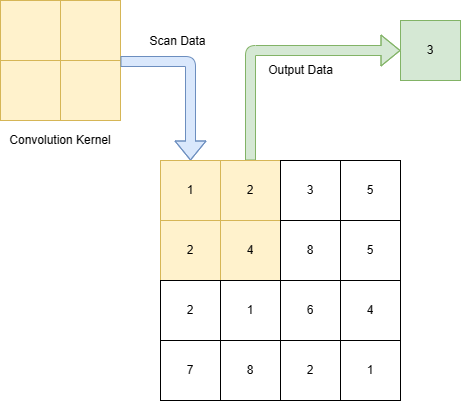
\includegraphics[scale=0.4] {PNG/2-8.png}
    \caption{Convolution kernel schematic}
    \label{fig:2-8}
\end{figure}

    \item Stride

Stride refers to the distance that the convolution kernel moves each time it is scanned in a certain direction. The setting of the stride should be determined in combination with the convolution kernel and the data situation. In the case of a very large dataset, a stride that is too small may not be able to extract the corresponding information quickly and effectively. However, in the case of limited data size, a stride that is too large may result in the discarding of many effective data.

\begin{figure}
    \centering
    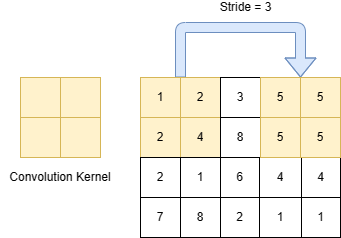
\includegraphics[scale=0.6] {PNG/2-9.png}
    \caption{Stride schematic}
    \label{fig:2-9}
\end{figure}

    \item Padding

Padding refers to adding meaningless all-zero or all-one data around the data when performing convolution scanning because the data on edge cannot be convolved separately by the convolution kernel. In order to effectively analyze the edge data, it is necessary to add padding around the data so that the convolution kernel can effectively scan the edge-related data.

\begin{figure}
    \centering
    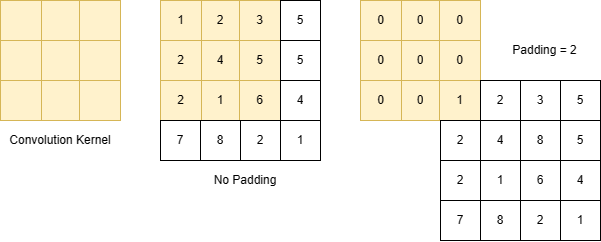
\includegraphics[scale=0.4] {PNG/2-10.png}
    \caption{Padding schematic}
    \label{fig:2-10}
\end{figure}

    \item Group

Convolution layers can also be grouped to train an input result simultaneously. For example, when the groups are set to 2, it is equivalent to having two convolution layers, each of which calculates half of the input channels and produces half of the output channels. Finally, the relevant results are merged to obtain a complete output.

\begin{figure}
    \centering
    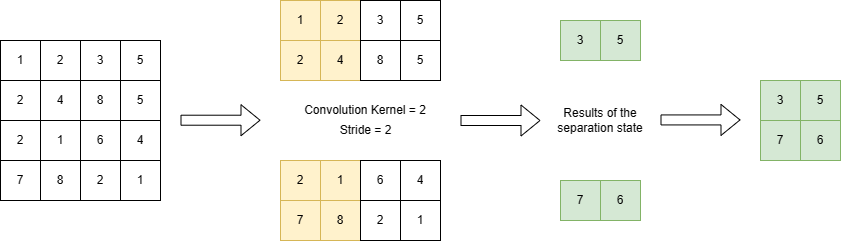
\includegraphics[scale=0.3] {PNG/2-11.png}
    \caption{Group training schematic}
    \label{fig:2-11}
\end{figure}

    \item Deconvolution

In generating content using convolution, related deconvolution techniques are also used. That is, by reversing convolution techniques, the data can be expanded reversely.

\begin{figure}
    \centering
    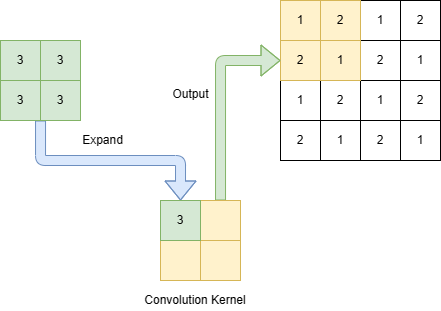
\includegraphics[scale=0.5] {PNG/2-12.png}
    \caption{Deconvolution schematic}
    \label{fig:2-12}
\end{figure}

\end{enumerate}

\subsubsection{Batch}

Batch processing technology solves the problem of data processing and model optimization adjustment. The batch size determines how much data are analyzed and processed before optimizing the model. The size of the batch directly affects the generation of model weights. A batch that is too large will affect the use of memory, while a batch that is too small will make the advantage of batch processing ineffective. Therefore, choosing a suitable batch size requires corresponding adjustment and optimization in application operations.

\subsection{Introduction to Speech Signal Processing}

A speech signal is an analog signal. Unlike image signals, speech signals require feature analysis and preprocessing during acquisition. For GANs to effectively process related data, the data being processed must have sufficient feature characteristics. Therefore, carrying out reasonable preprocessing work on speech signals is extremely important.

Speech is a time-varying signal, and the characteristics of phonemes within it are constantly changing. The original speech signal needs to be truncated into small segments in processing speech signals. Within each segment, the speech signal remains stable. The window used to truncate the segment is called a frame, and the segments obtained by sliding the window over the speech signal are called frames. This truncation operation is called windowing.

The windowing operation also requires precise control over the frame length. Each frame should contain a complete phoneme, while microscopically, it should have enough vibration cycles to ensure faithful Fourier transform computations. The frame length should not be too long, which would result in an unstable signal with too much information, nor too short, resulting in a low-resolution Fourier analysis with insufficient information.

However, it is impossible to obtain a complete periodic function in windowing operations. In many cases, overlapping features may occur between frames, resulting in noise that directly affects the effectiveness of subsequent computations. Therefore, to emphasize the information obtained in windowing and reduce noise, a filter is added to the target waveform during windowing to weaken the content at the two ends of each frame. This is beneficial for emphasizing the main content and obtaining better results in Fourier transforms.

However, important and valid information exists in the overlapping features we eliminate. In that case, blind filtering can lead to information loss. Therefore, overlap sampling is also performed in windowing operations, which reduces the sliding distance and ensures that each part of the content can be independently and effectively analyzed.

The features of speech signals mainly reside in the frequency domain. Thus it is necessary to transform the speech signal into the frequency domain for corresponding analysis. Three main types of frequency domain transformation methods exist filter bank methods, Fourier spectrum analysis algorithms derived from Fourier transform, and related algorithms derived from Mel-frequency spectra.

Filter bank methods are one of the earliest frequency spectrum analysis methods adopted. Its use is simple and robust. The core approach is extracting corresponding frequency information by filtering the digital model through multiple filters. Fourier spectrum analysis is studied through Fourier transform and short-time analysis of signals, with the core being a short-time fast Fourier transform. Mel-frequency spectrum transformation is the latest spectrum model designed based on auditory psychological characteristics of speech. Its analysis content is more in line with human perception \cite{15}.

As speech signals have language-specific features, some corresponding feature extraction algorithms have also been developed to recognize speech effectively. Currently, mainstream speech feature extraction algorithms include Mel frequency cepstral coefficients (MFCC), linear predictive coefficients (LPC), linear predictive cepstral coefficients (LPCC), discrete wavelet transform (DWT), and others \cite{16}. These speech feature extraction algorithms can effectively filter and recognize important features of speech, thereby accelerating speech analysis and recognition ability. However, speech feature extraction is not suitable for speech synthesis work because it needs more details, resulting in synthesized signals only exhibiting basic phonemic features but not complete speech features.

\section{Model Design and Validation}

\subsection{Model Design Preparation}

As larger batch training requires a significant amount of G-RAM, it is difficult to conduct experiments on a regular home computer. Even the entry-level Jetson Nano by NVIDIA cannot meet the experimental requirements. Therefore, cloud servers were used as the final experimental platform. The experimental machine was loaded with CUDA 1.10.0, Intel Xeon Cascade Lake (2.5 GHz), and NVIDIA T4 graphics card (8G). 

The speech database used in this study is the THCHS30 database from Tsinghua University, and 5273 sets of data were used for the experiments. All speech files are in 256kbps format and have a 16000Hz sampling rate, with a source format of 16-bit integers. The audio was subjected to normalization and limit processing, with an upper limit of 20dB and a lower limit of -100 dB. At the same time, windowing was performed during the preprocessing of speech files, with a window number of 2048 and a window length of 120ms. The files were written and stored in NumPy format. The stored data includes the raw speech time domain data and the speech frequency domain data transformed by Mel-spectrogram. 

The analyzed data was classified and stored during the preprocessing stage to store the experimental data properly. Firstly, train and test folders were created to store the training and testing files. Audio and mel folders were also created to store the encoded raw waveform files and their corresponding transformed spectrogram files.

In the middle of the training phase, the logdir folder was established using the parameter-saving feature in torch, which stores the training results and related parameters after each training cycle. If the related parameters exist, the training continues to generate results. However, if the related parameters do not exist, they are re-generated.

\begin{lstlisting}[caption={File Tree}, label={lst:3-1}]
Main
├── Training
│   ├── Data
│   │   ├── Time-Domain
│   │   └── Frequency-Domain
│   └── Test
│       ├── Time-Domain
│       └── Frequency-Domain
└── Log
\end{lstlisting}

\subsection{GAN Modeling}

\subsubsection{Generator Design}

This paper's generator comprises seven independent blocks and two residual convolution structures. Each independent block is named GBlock and consists of four stacks. Using multiple independent blocks effectively reduces the workload, allowing the focus to be on the design of the independent blocks rather than the overall network design. Before entering the GBlock layer, a one-dimensional convolutional layer is added to the model for basic data preprocessing to adapt it to its computational dimensions. In the post-processing stage, data is organized and corrected through a one-dimensional convolutional layer and a tanh activation function.

\begin{figure}
    \centering
    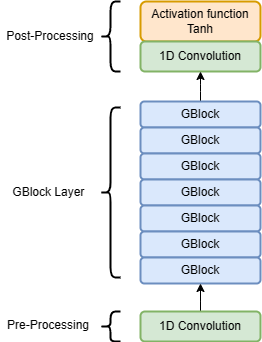
\includegraphics[scale=0.7] {PNG/3-2.png}
    \caption{Generator structure diagram}
    \label{fig:3-2}
\end{figure}

To adapt to the trend of continuously biased global optimization conditions in convolution, the four-layer convolution kernel is set with continuously expanding dilation factors: 1, 2, 4, and 8 to control the size of the holes, thereby obtaining an appropriate convolution kernel. The continuously expanding dilation factor allows the convolution kernel to expand continuously, thereby obtaining a larger field of view and a more global visual range. This can help capture more macroscopic data characteristics, and pay more attention to overall feature details in the later processing stage, rather than being limited to minor details, thereby avoiding pattern collapse.

\begin{table}[ht]
\centering
\caption{Generator GBlock Module Data Sheet}
\label{tab:3-1}
\begin{tabularx}{0.5\textwidth}{|X|X|X|X|X|}
\hline
  Module Name & Input Channel & Output Channel & Noise Channel & UpSampling Factor \\
\hline
  GBlock1 & 768 & 768 & 128 & 1 \\
\hline
  GBlock2 & 768 & 768 & 128 & 1 \\
\hline
  GBlock3 & 768 & 384 & 128 & 2 \\
\hline
  GBlock4 & 384 & 384 & 128 & 2 \\
\hline
  GBlock5 & 384 & 384 & 128 & 2 \\
\hline
  GBlock6 & 384 & 192 & 128 & 3 \\
\hline
  GBlock7 & 192 & 96 & 128 & 5 \\
\hline
\end{tabularx}
\end{table}

Each GBlock in this study was designed with four similar stacks, augmented with a two-level residual network and batch normalization operations. Each stack consists of a ReLU activation function followed by a one-dimensional convolution. In particular, the first stack contains an upsampling module between the activation function and convolution, which corrects the issue of the output frequency being smaller than the input frequency. The generator convolutions mainly used dilated convolutions to increase the receptive field of the convolution kernel by filling in the gaps between convolution kernels, maximizing the retention of details, and avoiding the loss of edge features. Additionally, a two-level residual network was incorporated into the design to ensure no excessive gradient disappearance problem during the later training process. Each stack underwent batch normalization operations to adjust the input data and help the neural network learn the rules in the data, preventing undesirable data from interfering with the training of the activation function and convolution module.

\begin{figure}
    \centering
    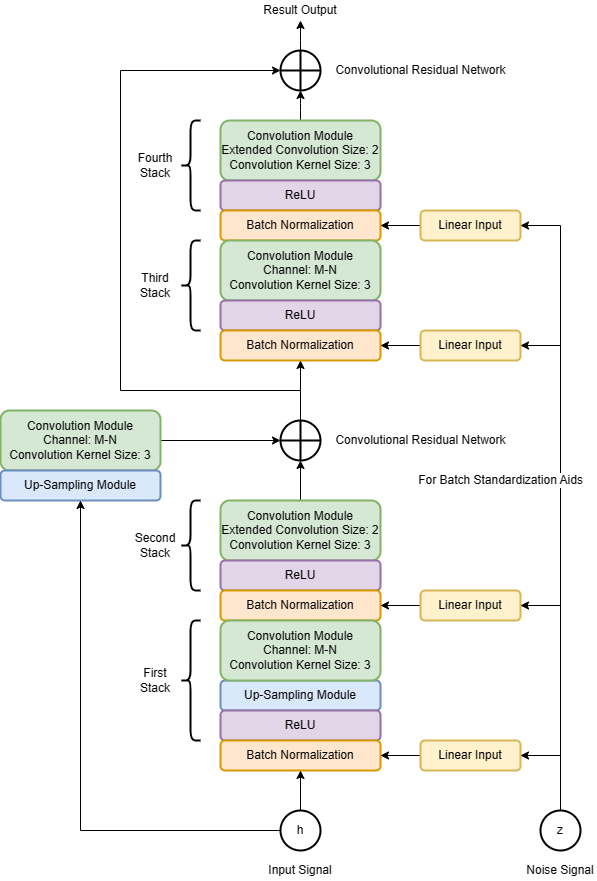
\includegraphics[scale=0.44] {PNG/3-3.png}
    \caption{Structure of GBlock \cite{17}}
    \label{fig:3-3}
\end{figure}

\subsubsection{Discriminator}

The discriminator in this work was designed using the SN-GAN model \cite{18}. Each convolutional layer consists of a one-dimensional layer based on mel-spectrogram analysis and a leaky activation function.

\begin{figure}
    \centering
    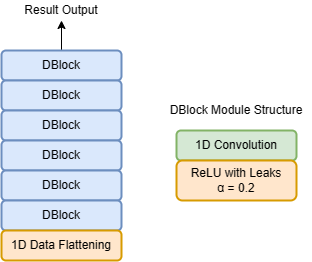
\includegraphics[scale=0.7] {PNG/3-4.png}
    \caption{Discriminator and DBlock Structures}
    \label{fig:3-4}
\end{figure}

Unlike the generator, the model does not use convolutional layers to prepare the data; instead, it simply flattens the data in one dimension to preserve the maximum data details. Then, seven independent DBlocks were stacked to improve the efficiency of the development process. The model adjusts the weight function with a normalization factor $\alpha$ to bias the optimization towards more stable situations. The default value for the activation function $\alpha$ is set to 0.2. The convolutional kernel parameters were set with corresponding dilation factors to expand their visual fields continuously. They tended to train on global features in the later stages to prevent mode collapse.

\begin{table}[ht]
\centering
\caption{Discriminator and DBlock Data Sheet}
\label{tab:3-2}
\begin{tabularx}{0.5\textwidth}{|X|X|X|X|X|X|X|}
\hline
  Module Name & Input Channel & Output Channel & Convo-lution Kernel & Stride & Padding & Group \\
\hline
  Conv1d-1 & 1 & 16 & 15 & 1 & / & 1 \\
\hline
  Conv1d-1 & 16 & 64 & 41 & 4 & 20 & 4 \\
\hline
  Conv1d-1 & 64 & 256 & 41 & 4 & 20 & 16 \\
\hline
  Conv1d-4 & 256 & 1024 & 41 & 4 & 20 & 64 \\
\hline
  Conv1d-5 & 1024 & 1024 & 41 & 4 & 20 & 256 \\
\hline
  Conv1d-6 & 1024 & 1024 & 5 & 1 & 2 & 1 \\
\hline
  Conv1d-7 & 1024 & 1 & 3 & 1 & 1 & 1 \\
\hline
\end{tabularx}
\end{table}

\subsection{Optimizer \& Loss Function Design}

The generator and discriminator employ the popular Adam optimizer with a small default learning rate to ensure reasonable parameter adjustment and prevent oscillation \cite{19}. The loss function used for the first two training steps of the discriminator is MSELoss, and the final backward calculation loss is the sum of the loss values obtained from real and fake data.

\begin{align}
    Loss_D = Loss_{RealData} + Loss_{FakeData}
\end{align}

The loss design for the generator is more complex. Two different frequency-based loss functions are used to calculate the generator's loss. The design incorporates both GAN ideas and the idea of comparing generated data directly with original data to obtain the loss:

\begin{enumerate}
    \item The discriminator calculates the loss function, $Loss_D$, based on the generated data from the generator.

    \item The generated data and original data are compared from a frequency domain perspective. One method involves calculating the spectral norm, while the other uses the mean absolute error loss function to calculate two log-compressed values.

    \item The generator's loss function, $Loss_G$, is calculated by combining the discriminator optimization parameter $(\lambda_{adv})$ that is set. In this experiment, $(\lambda_{adv})$ is set to 4 by default.
\end{enumerate}

\begin{align}
    Loss_{SpectralConvergence} = \frac{||message_{target} - message_{generate}||}
                                      {||message_{target}||}
\end{align}

\begin{equation}
    \begin{aligned}
        Loss_{LogSTFTMagnitude} = \\ \frac{\sum_{i=1}^{n} {|\log{(message_{target})} - \log{(message_{generate})}|}} {n}
    \end{aligned}
\end{equation}

\begin{align}
    Loss_G = Loss_D \times lambda_{adv} + Loss_{SC} + Loss_{Mag}
\end{align}

\subsection{Fine-Tune \& Final Design}

One of the key considerations during training is the choice of batch size. The batch size directly affects the optimization direction and the strength of the optimization. A too-small batch can result in a wrong direction or insufficient optimization strength. At the same time, a batch that is too large can lead to high memory requirements or insufficient optimization strength. In the early model design stage, batch sizes below ten were used. Tests have shown that a too-small batch can only exacerbate convergence oscillations or even affect normal convergence. Based on the test results, a batch size of 30 can still achieve good convergence. However, it requires a longer training period to manifest, and the optimization effect is also very significant. For example, during the initial warm-up training of 20,000 steps, if a batch size of 8 is used, the loss can only converge to around 1.6 with significant oscillations. The convergence trend could be clearer and easier to continue. However, with a batch size of 30, the loss can converge significantly to around 1.5 with a clear convergence process. Batch sizes above 15 also exhibit good convergence properties. From the perspective of computation time, the computation time for batch sizes before 20 is stable at around 0.5 seconds per step, while the computation time for a batch size of 30 increases significantly to around 1 second per step. This test result indicates that the computational power is far beyond the batch size requirements, and the main problem lies in the size of memory. Considering the convergence requirements, training time, and computation cost, the final batch size is 15. This choice considers the overall convergence requirements, training time, and computation cost.

\begin{figure}
    \centering
    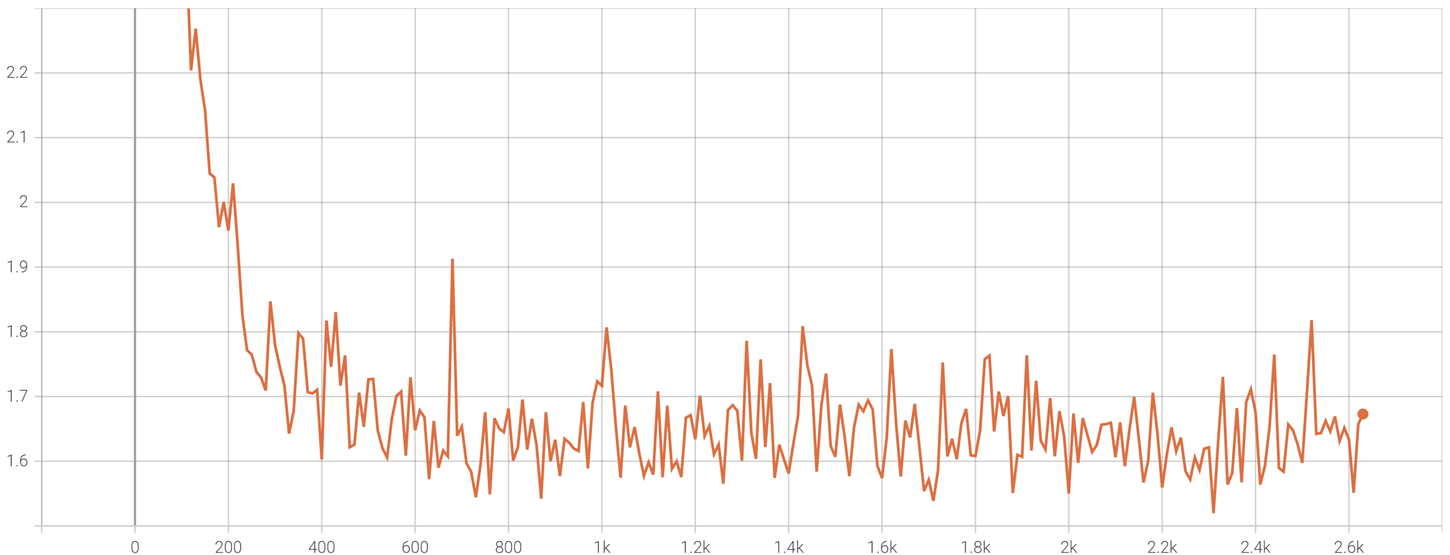
\includegraphics[scale=0.6] {PNG/3-5.png}
    \caption{batch=8 g loss graph}
    \label{fig:3-5}
\end{figure}

\begin{figure}
    \centering
    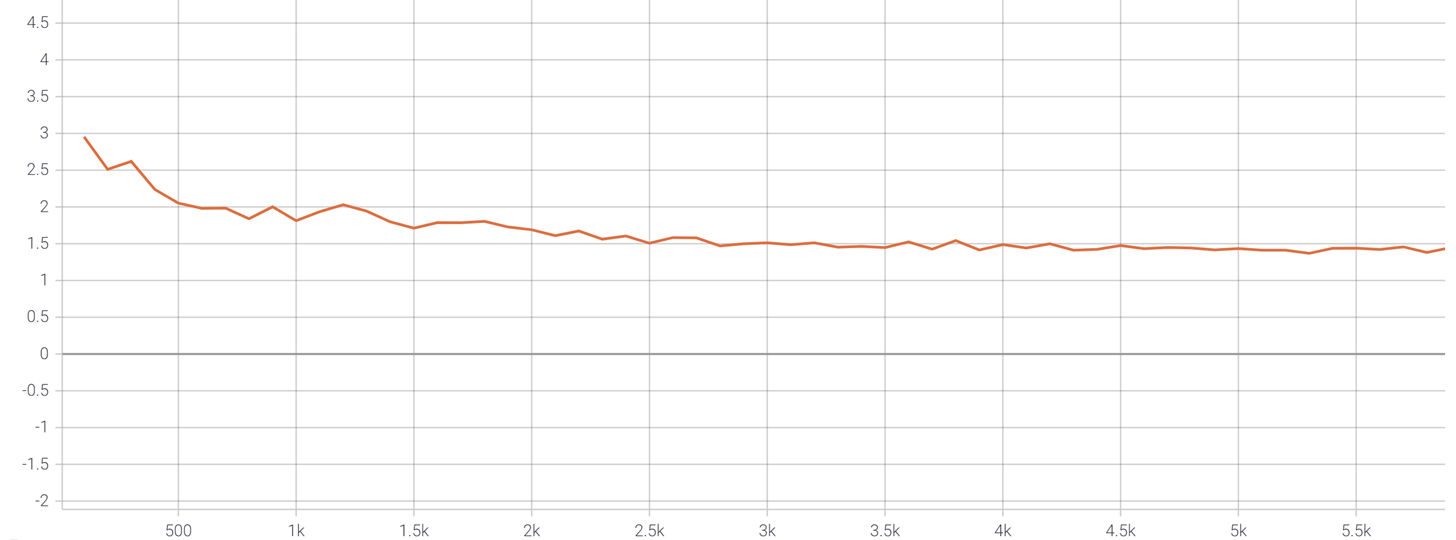
\includegraphics[scale=0.6] {PNG/3-6.png}
    \caption{batch=30 g loss graph}
    \label{fig:3-6}
\end{figure}

Secondly, due to the rapid growth of the discriminator, it is necessary to perform pre-warm-up training for the generator to achieve a better adversarial balance. If the discriminator is added too early with enough pre-training time, it will result in better convergence. Therefore, a long pre-training period is necessary before the training process to enable the generator to counter the discriminator effectively. Testing data reveals that when the batch size is eight and the discriminator is added after 50 steps, the discriminator grows too fast, causing the generator to crash. The generator loss exhibits severe oscillations with some convergence tendency. However, when the discriminator is added after a delay, significant convergence is observed in the early stages, and rapid convergence is observed later. Data from adding the discriminator after 200 steps shows a clear convergence tendency in the early stages. The amplitude of oscillations starts to converge after the discriminator is added. However, significant oscillations still occur later, though there is a clear overall convergence trend. This suggests that the overall pre-training time still needs to be improved, and more pre-training is needed to prepare for subsequent training.

\begin{figure}
    \centering
    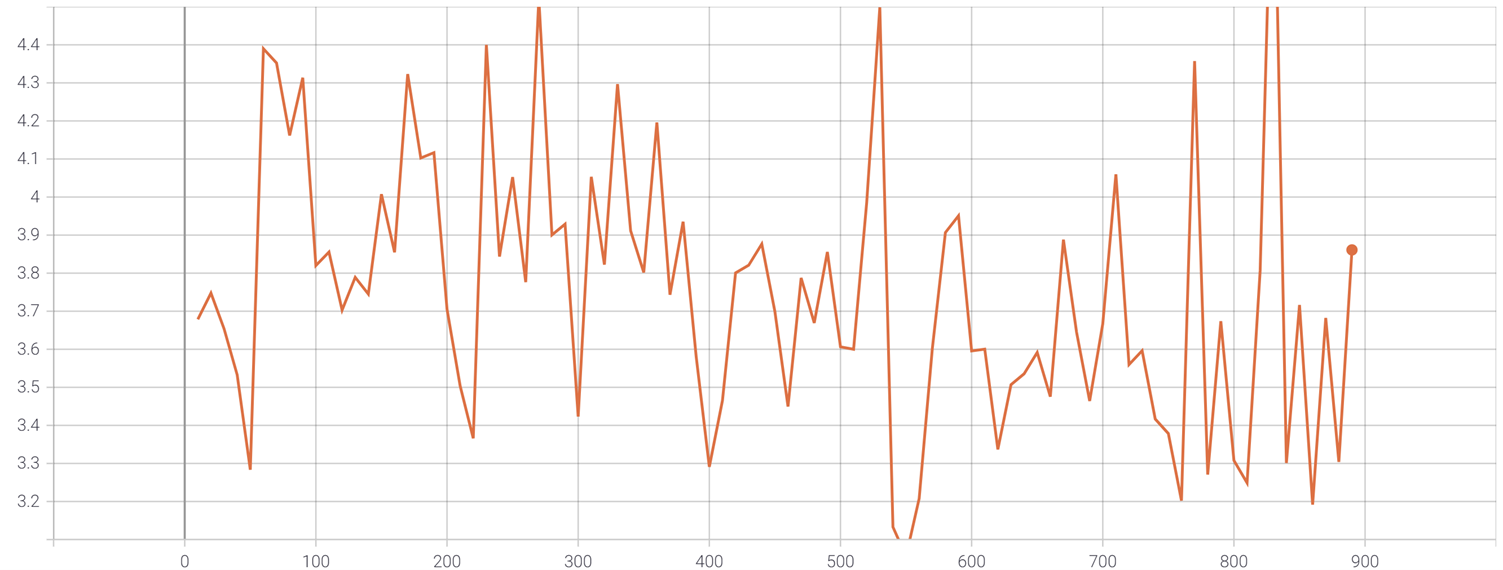
\includegraphics[scale=0.6] {PNG/3-7.png}
    \caption{Introduce discriminator at 50 steps g loss graph}
    \label{fig:3-7}
\end{figure}

\begin{figure}
    \centering
    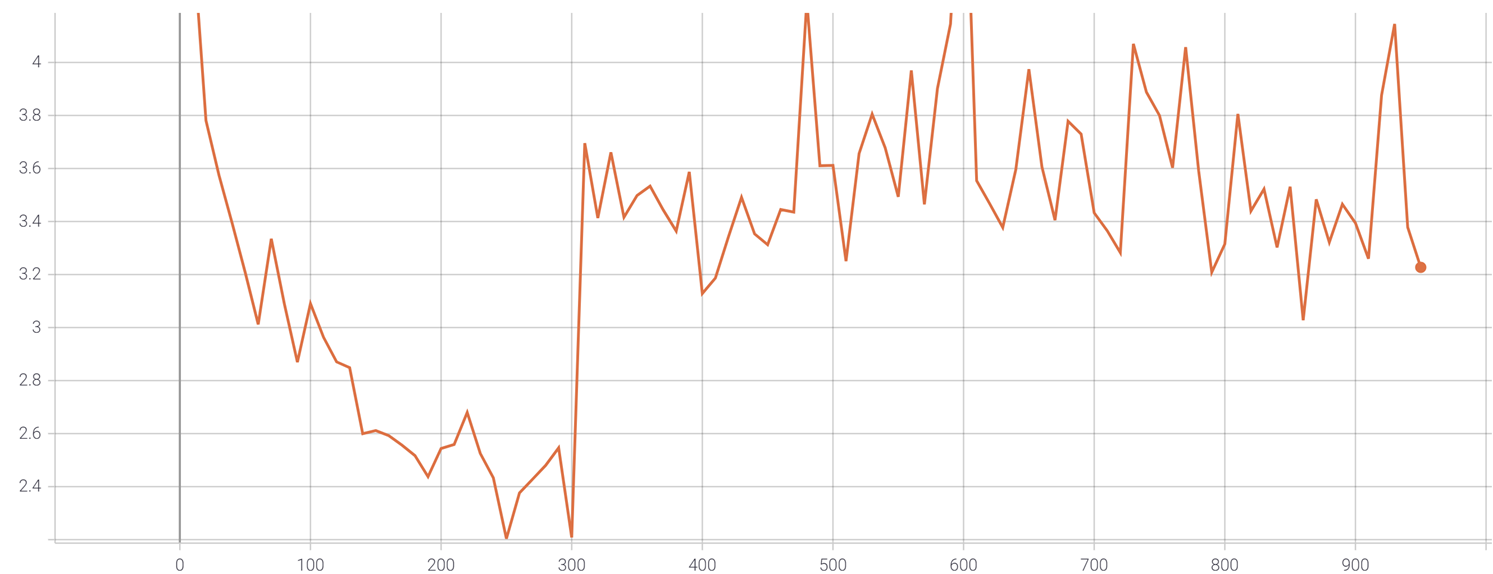
\includegraphics[scale=0.6] {PNG/3-8.png}
    \caption{Introduce discriminator at 200 steps g loss graph}
    \label{fig:3-8}
\end{figure}

The final chosen configuration involves setting the batch size to 15 and setting the discriminator's learning rate and the generator's 0.0001. The generator is added after 20,000 steps, and the lambda value is set to 4. The training process involves 300,000 steps. Throughout the training process, adversarial conditions are monitored to prevent training collapses.

\section{Results \& Effect Analysis}

\subsection{Loss Function Analysis}

From the loss of the discriminator, we can observe that the system is still in a state of balanced opposition after introducing the discriminator. Both the loss value of the synthetic data and the real data exhibit some oscillation, but it is a relative oscillation. Therefore, when combining the d loss value, a good convergence effect can be achieved towards 0.5. Both data sets from the discriminator converge to 0.25, indicating an ideal performance according to the expected mean squared error loss function. This suggests that the overall adversarial conditions are well-balanced, demonstrating that the model still possesses strong vitality and stability. The adv loss serves as an overall evaluation of the discriminator, which remains very low and shows minimal fluctuations after introducing the discriminator. This indicates that its corrective ability towards the generator has remained stable and reliable, continuously providing optimization power for the generator. Overall, the discriminator's situation demonstrates the GAN model's feasibility and reliability.

\begin{figure}
    \centering
    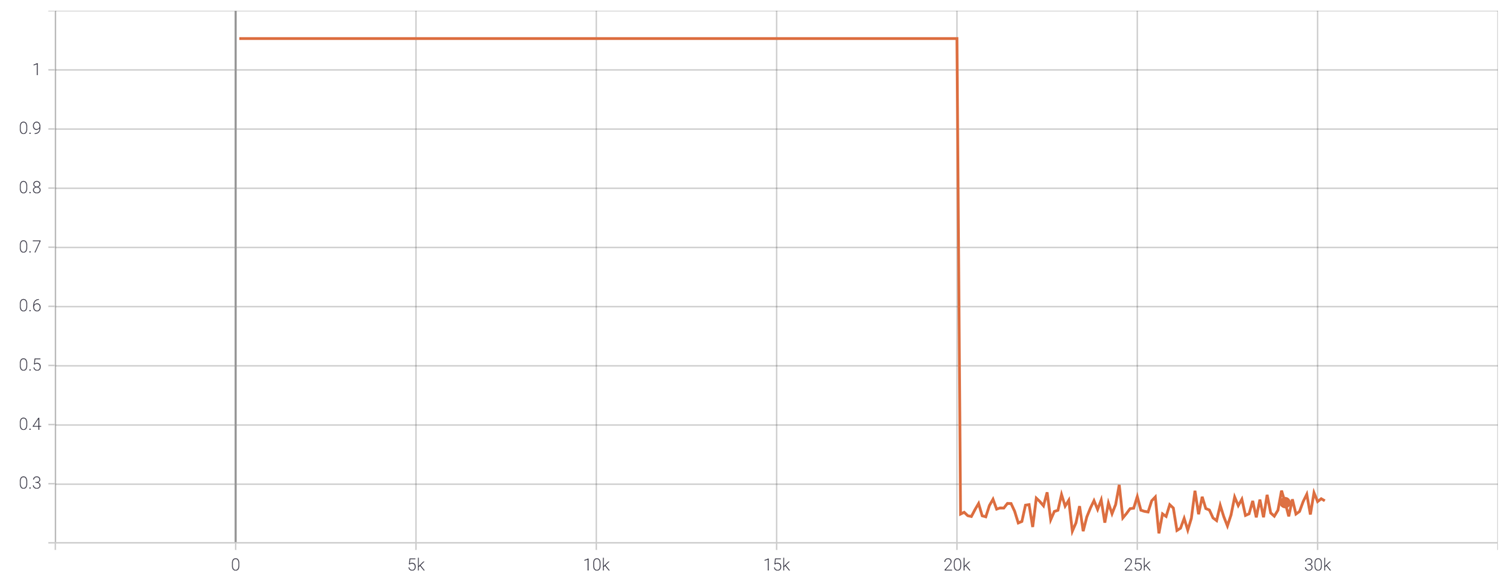
\includegraphics[scale=0.6] {PNG/4-1.png}
    \caption{adv loss graph}
    \label{fig:4-1}
\end{figure}

\begin{figure}
    \centering
    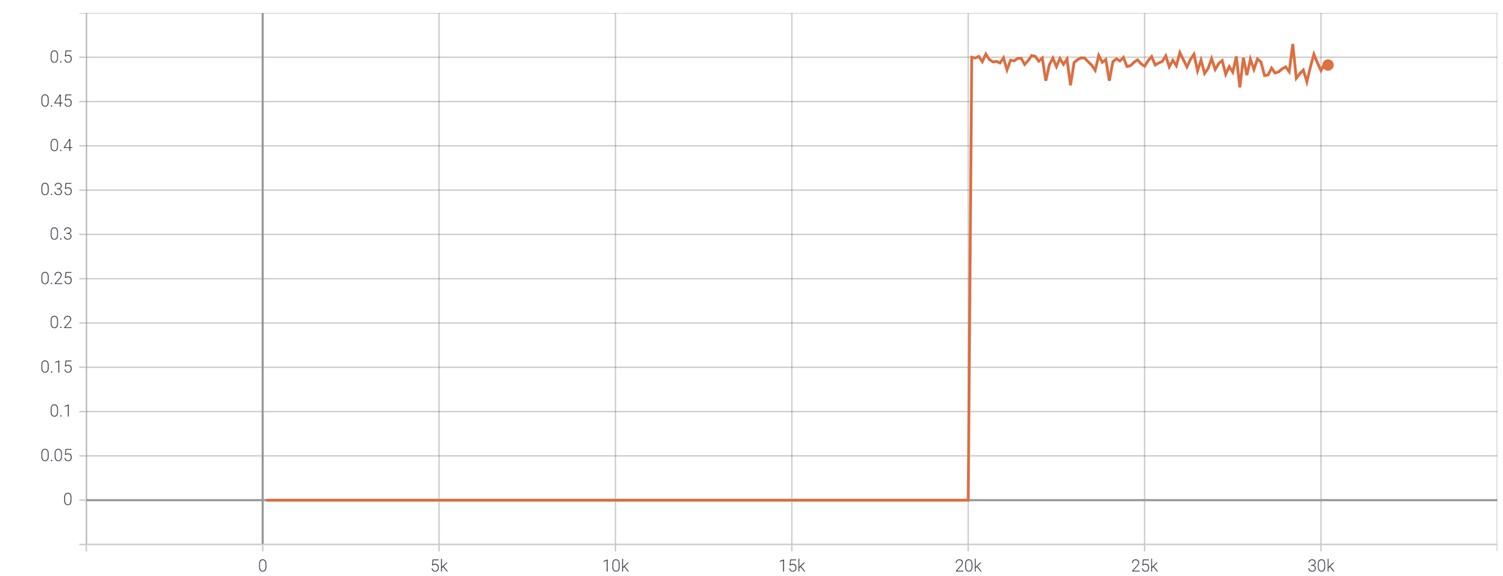
\includegraphics[scale=0.6] {PNG/4-2.png}
    \caption{d loss graph}
    \label{fig:4-2}
\end{figure}

\begin{figure}
    \centering
    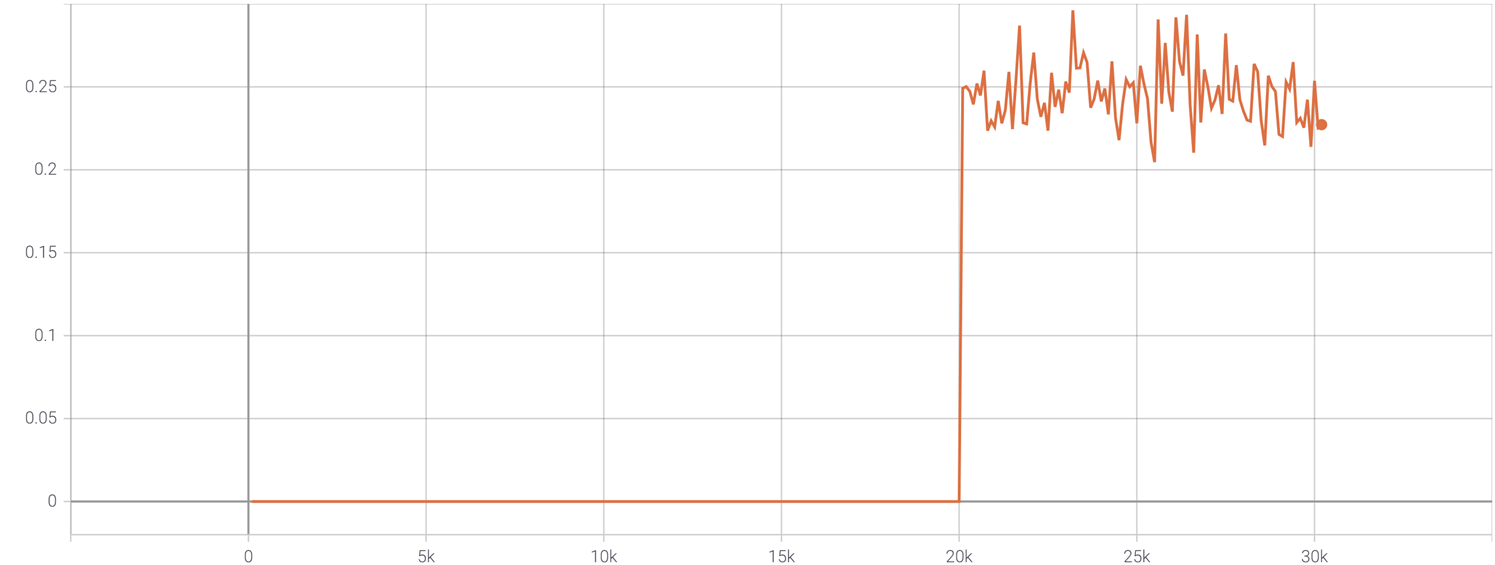
\includegraphics[scale=0.6] {PNG/4-3.png}
    \caption{fake loss graph}
    \label{fig:4-3}
\end{figure}

\begin{figure}
    \centering
    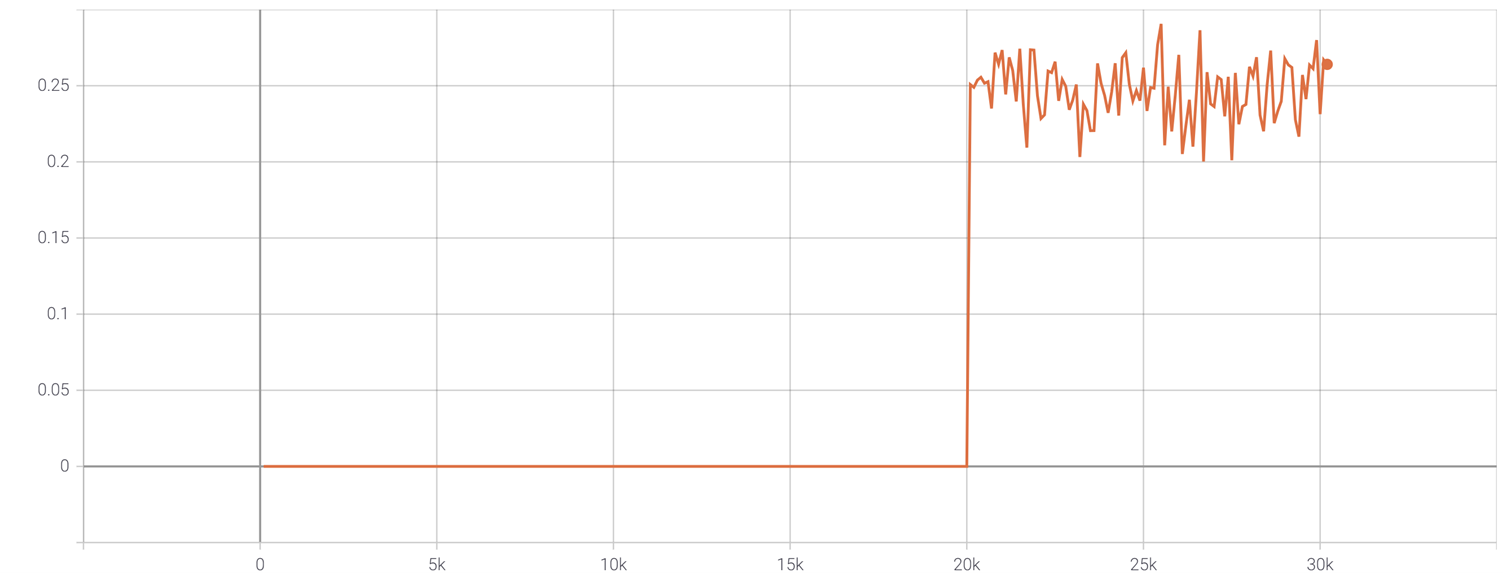
\includegraphics[scale=0.6] {PNG/4-4.png}
    \caption{real loss graph}
    \label{fig:4-4}
\end{figure}

The generator maintained a good convergence trend in the early preheating training. It continued to perform well after the discriminator was introduced. The g loss rebounded to a high level with the introduction of the mid-term GAN framework but still maintained a state of convergence. Both mag loss and sc loss showed a stable convergent trend, with their values converging to around 0.5, consistent with the expected stable loss functions.

The generator exhibited a very stable convergence trend in the early stage. The high-batch state provided sufficient preheating preparation for the overall convergent training. After the discriminator was introduced in the later stages of training, the generator's loss function exhibited noticeable oscillations but maintained a very stable convergence state. After introducing the discriminator, the mag loss remained stable at around 0.5 and generated a small, stable oscillation nearby. The sc loss showed larger oscillations but continued the pre-training convergence trend and remained very clearly convergent. The generator's loss demonstrates that the GAN model still has strong vitality in audio processing and can effectively promote model convergence, accelerate the overall speed and situation of convergence, and thus produce good synthesized speech.

\begin{figure}
    \centering
    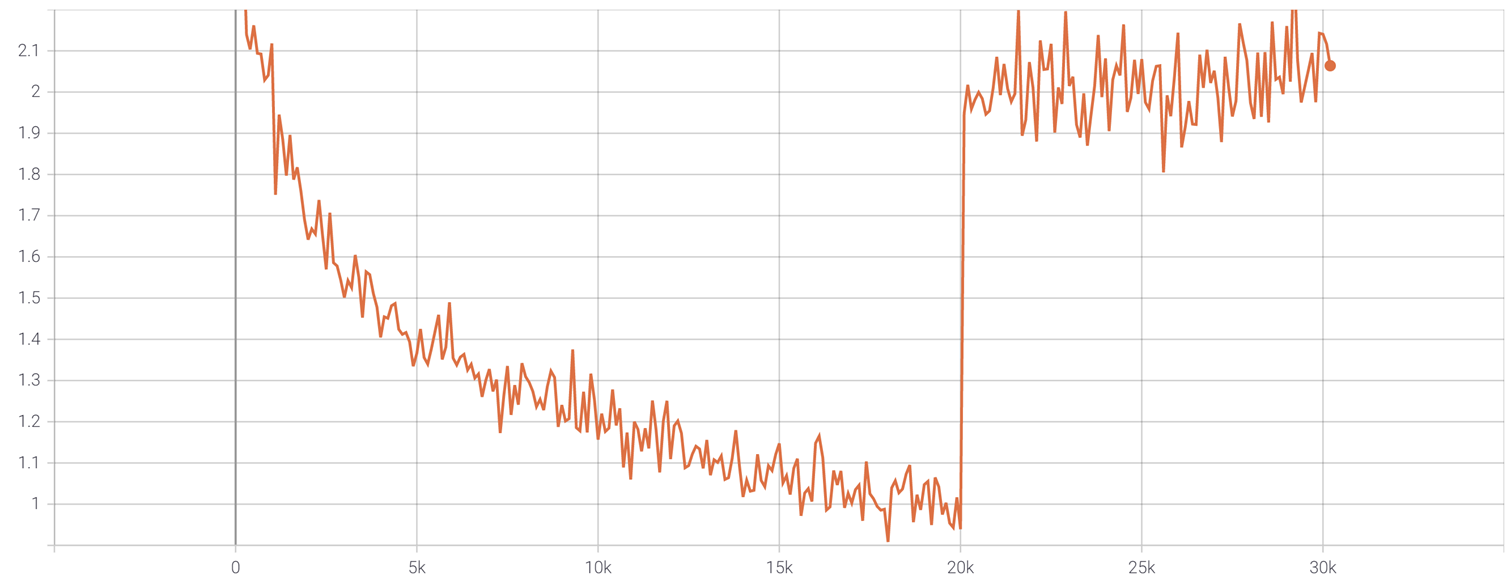
\includegraphics[scale=0.55] {PNG/4-5.png}
    \caption{g loss graph}
    \label{fig:4-5}
\end{figure}

\begin{figure}
    \centering
    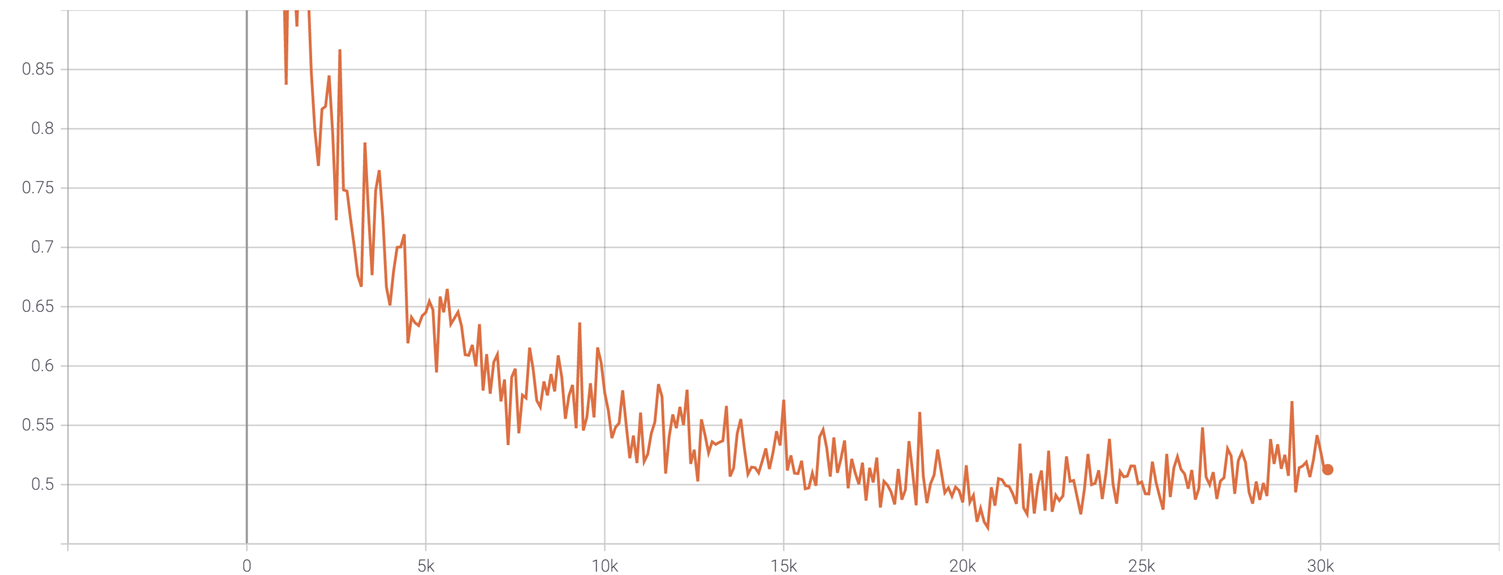
\includegraphics[scale=0.55] {PNG/4-6.png}
    \caption{mag loss graph}
    \label{fig:4-6}
\end{figure}

\begin{figure}
    \centering
    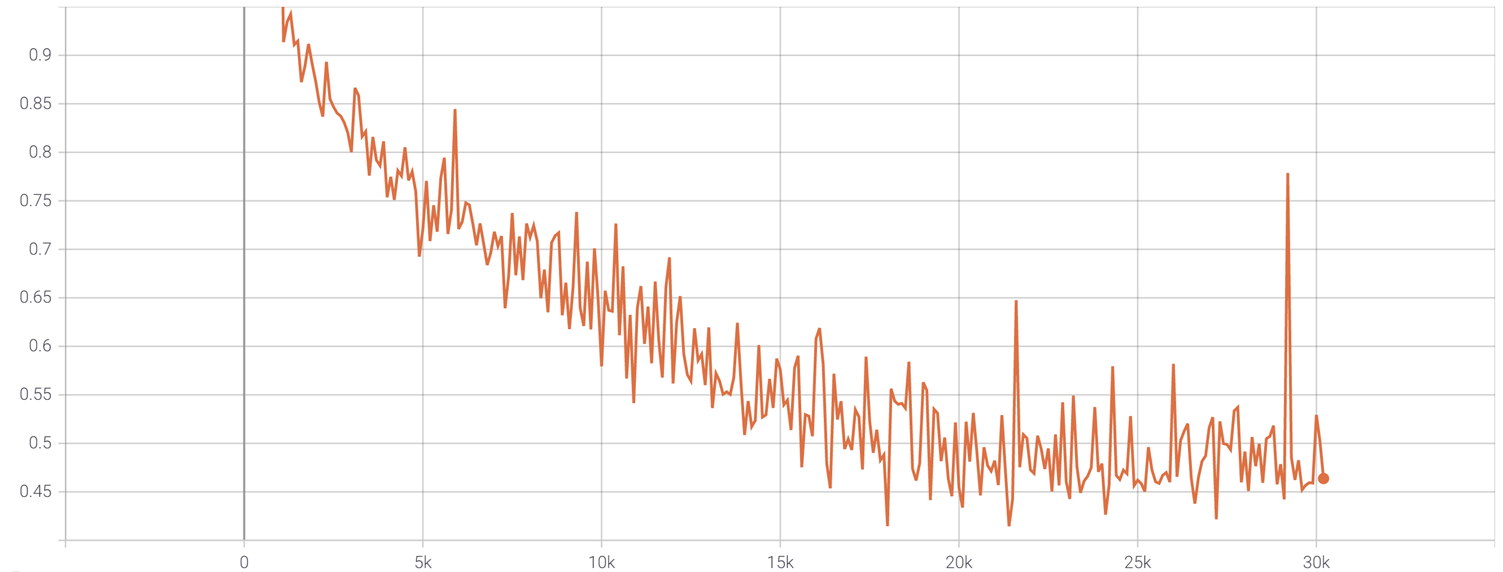
\includegraphics[scale=0.55] {PNG/4-7.png}
    \caption{sc loss graph}
    \label{fig:4-7}
\end{figure}

\subsection{Audio Generation Quality Analysis}

Objectively, the generated audio has restored the native waveform in the time domain and has corresponding audio features in the corresponding area. The amplitude of the audio has been weakened, but it does not affect the overall waveform similarity. The generated audio has restored the semantic-related features in the frequency domain and coincides with the original speech spectrum. However, in the entire frequency domain, especially in the low-frequency part, a lot of noise information still needs to be eliminated, which affects the specific audio processing situation. Overall, the relevant features of speech have been very well restored, but the noise part of the details still needs to be trained more deeply. From a subjective perspective, the generated data spectrum has well simulated the speech and semantic content in the original file. The human ear can recognize more obvious timbre features and language content. However, the clarity features still need to be better restored, and there is still much noise.

\begin{figure}
    \centering
    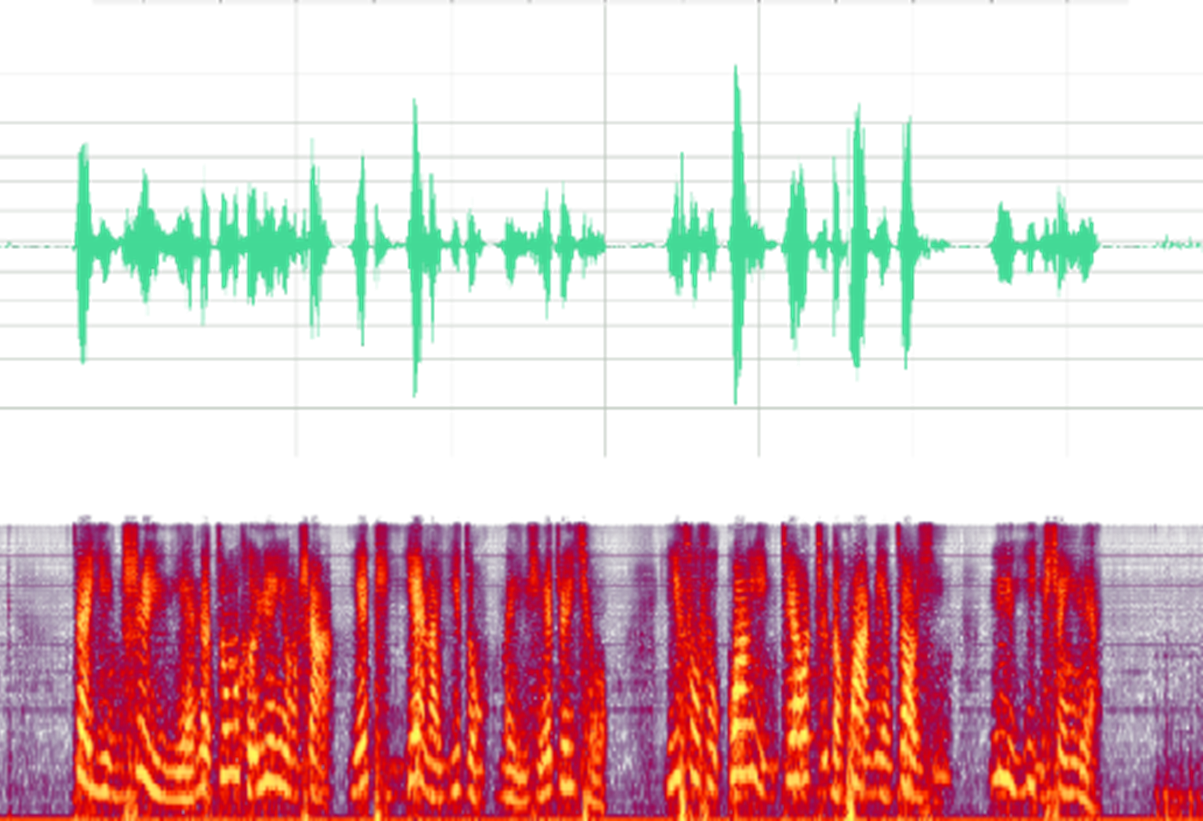
\includegraphics[scale=0.6] {PNG/4-8.png}
    \caption{Generated Spectrum}
    \label{fig:4-8}
\end{figure}

\begin{figure}
    \centering
    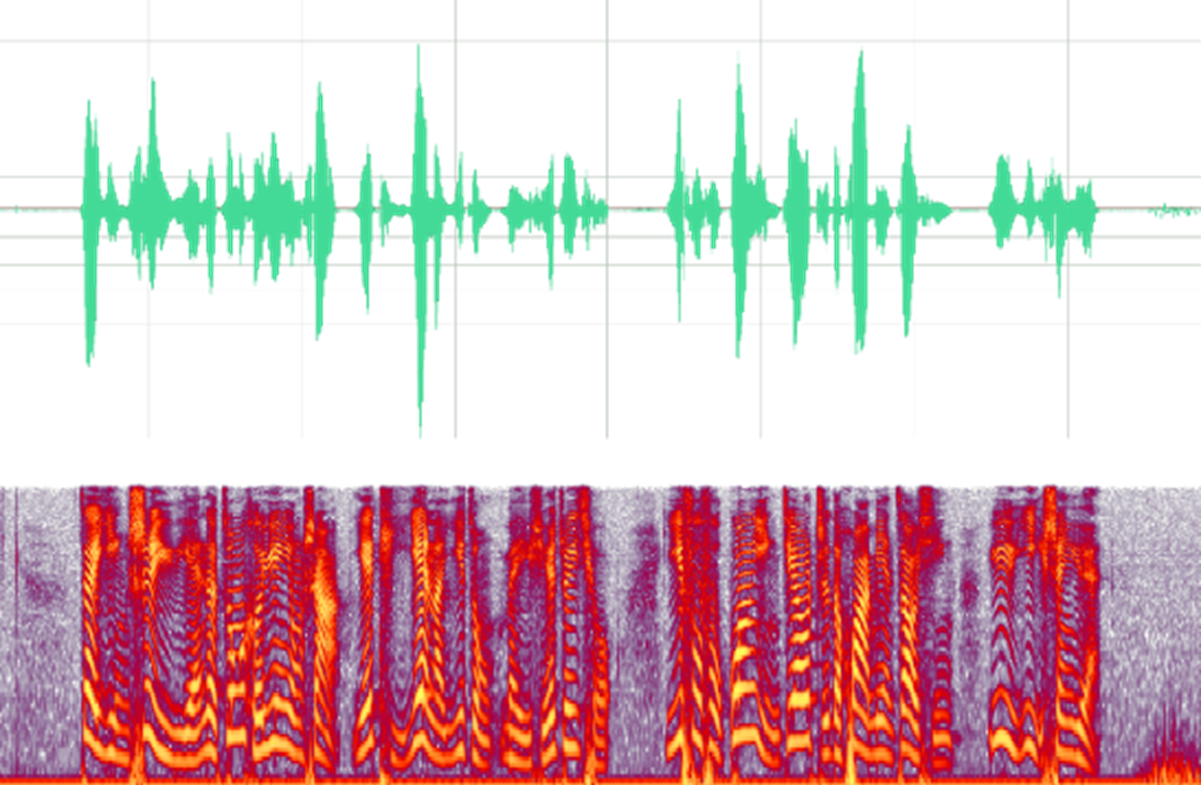
\includegraphics[scale=0.6] {PNG/4-9.png}
    \caption{Real Spectrum}
    \label{fig:4-9}
\end{figure}

\section{Conclusion}

As a new neural network deep learning model, Generative Adversarial Networks (GAN) have great potential for mining in neural network training. Currently, in China, training of GAN models is still in its early stages, and there is still much space for exploration waiting for researchers to explore. GAN also has tremendous potential in speech synthesis. Its core nature of adversarial unsupervised learning can help speed up the overall model convergence and achieve very good generation results. In addition, its tolerance for speech sets can greatly reduce the related work of speech pre-processing, making it easier to train a complete speech generation model. From a practical point of view, attention should be paid to pre-training and batch-related situations for GAN speech models. GAN speech models can achieve good generation results only in situations with sufficient pre-training and large enough batch sizes.

From a macro perspective, the design and development of GAN in speech synthesis still need improvement, and there is still much room for expansion and development in the existing models. The optimization and improvement consist of two aspects: the optimization of the audio preprocessing stage, how to extract feature operations more concisely using a superior performance data set with higher effective information and less data redundancy while not losing any useful information. The other aspect is the corresponding optimization of the training model. Designing more efficient audio models that facilitate overall training speed and efficiency improvement is essential. The digital signal processing and GAN research fields need efforts to collaborate and design better models.

\begin{CJK}{UTF8}{gbsn}

\bibliographystyle{IEEEtran}
\bibliography{Ref}

\end{CJK}
\end{document}
